% ------------------------------------------------------------------------
% file `travail_de_vacances-exercise-20-exercise-body.tex'
%   in folder `xsim/'
%
%     exercise of type `exercise' with id `20'
%
% generated by the `exercise' environment of the
%   `xsim' package v0.21 (2022/02/12)
% from source `travail_de_vacances' on 2022/10/11 on line 822
% ------------------------------------------------------------------------
    \begin{wrapfigure}{r}{.3\linewidth}
        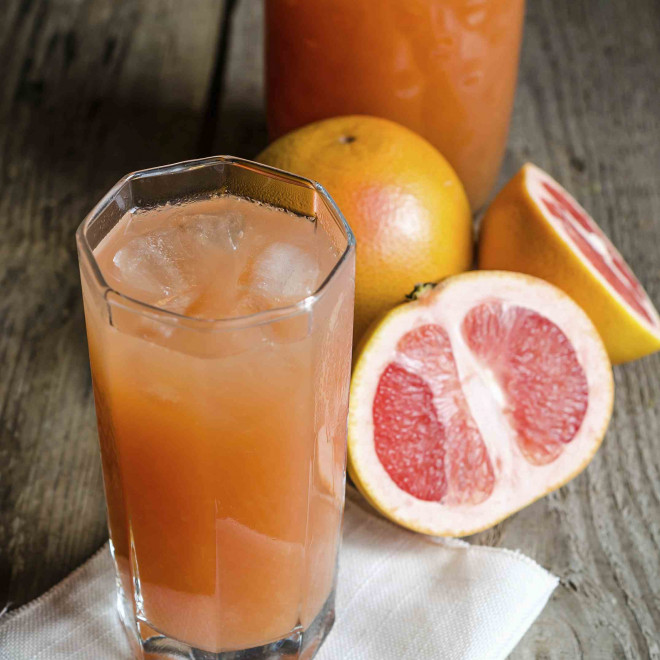
\includegraphics[width=\linewidth]{images/cocktail.jpg}
    \end{wrapfigure}
    Un délicieux jus de fruits frais est composé de :
    \begin{itemize}
        \item $\dfrac{2}{3}$ de jus d'oranges.
        \item $\dfrac{1}{3}$ de jus de pamplemousses.
    \end{itemize}

    Il faut presser \SI{1}{kg} d'oranges pour obtenir \SI{40}{cl} de jus et
    \SI{1}{kg} de pamplemousses pour obtenir \SI{25}{cl} de jus.\par
    Dans le commerce tu peux trouver des oranges et des pamplemousses au prix
    suivant :
    \begin{description}
        \item[Oranges] 12€/\SI{5}{kg}
        \item[Pamplemousses] 10,80€/\SI{4}{kg}
    \end{description}
    Que coûte la préparation de \SI{4,5}{l} de ce cocktail de fruis frais si
    tu achètes la quantité exacte de fruis ?
